\newpage
\section{Speedometer}
The purpose of the speedometer is to measure the car's current speed.

\subsection{Design}
The speed is measured using a TLE49X5L Hal sensor\cite{TLE4905}. This sensor has a digital output wich will go HIGH when a magnet is near the sensor. The voltage level for the HIGH output is equal to the supply voltage V\textsubscript{S}. As the sensor's output is to be measured by the PSoC, then a supply 5 V is used.
In order for the sensor to output a digital signal, it must be connected as seen in the circuit in \ref{fig:HAL_application} below.

\begin{figure}[H]
	\centering
	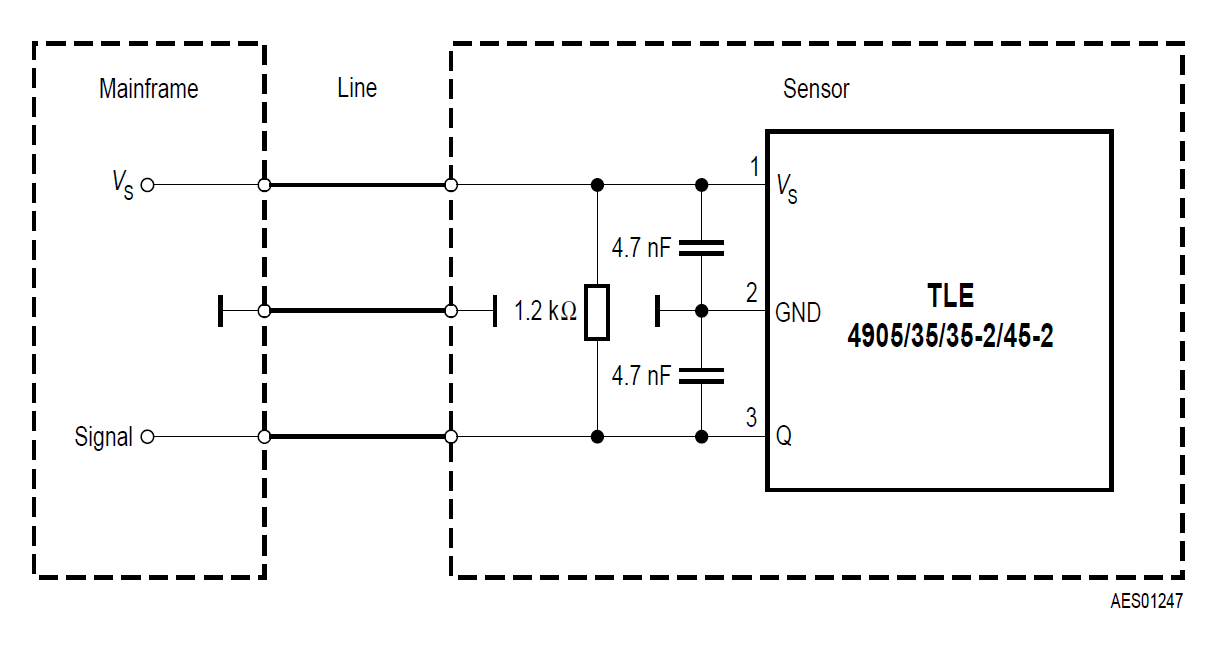
\includegraphics[width=0.6\linewidth]{Hardware/Pictures/HAL_Application}
	\caption{HAL-Sensor application circuit}
	\label{fig:HAL_application}
\end{figure}

The measured objects are magnets which are applied to each spoke of the car's wheel. By placing the sensor near the wheel, then the output signal can be used to measure the speed. A sketch of this configuration is shown in \ref{fig:Speed_sketch} below.

\begin{figure}[H]
	\centering
	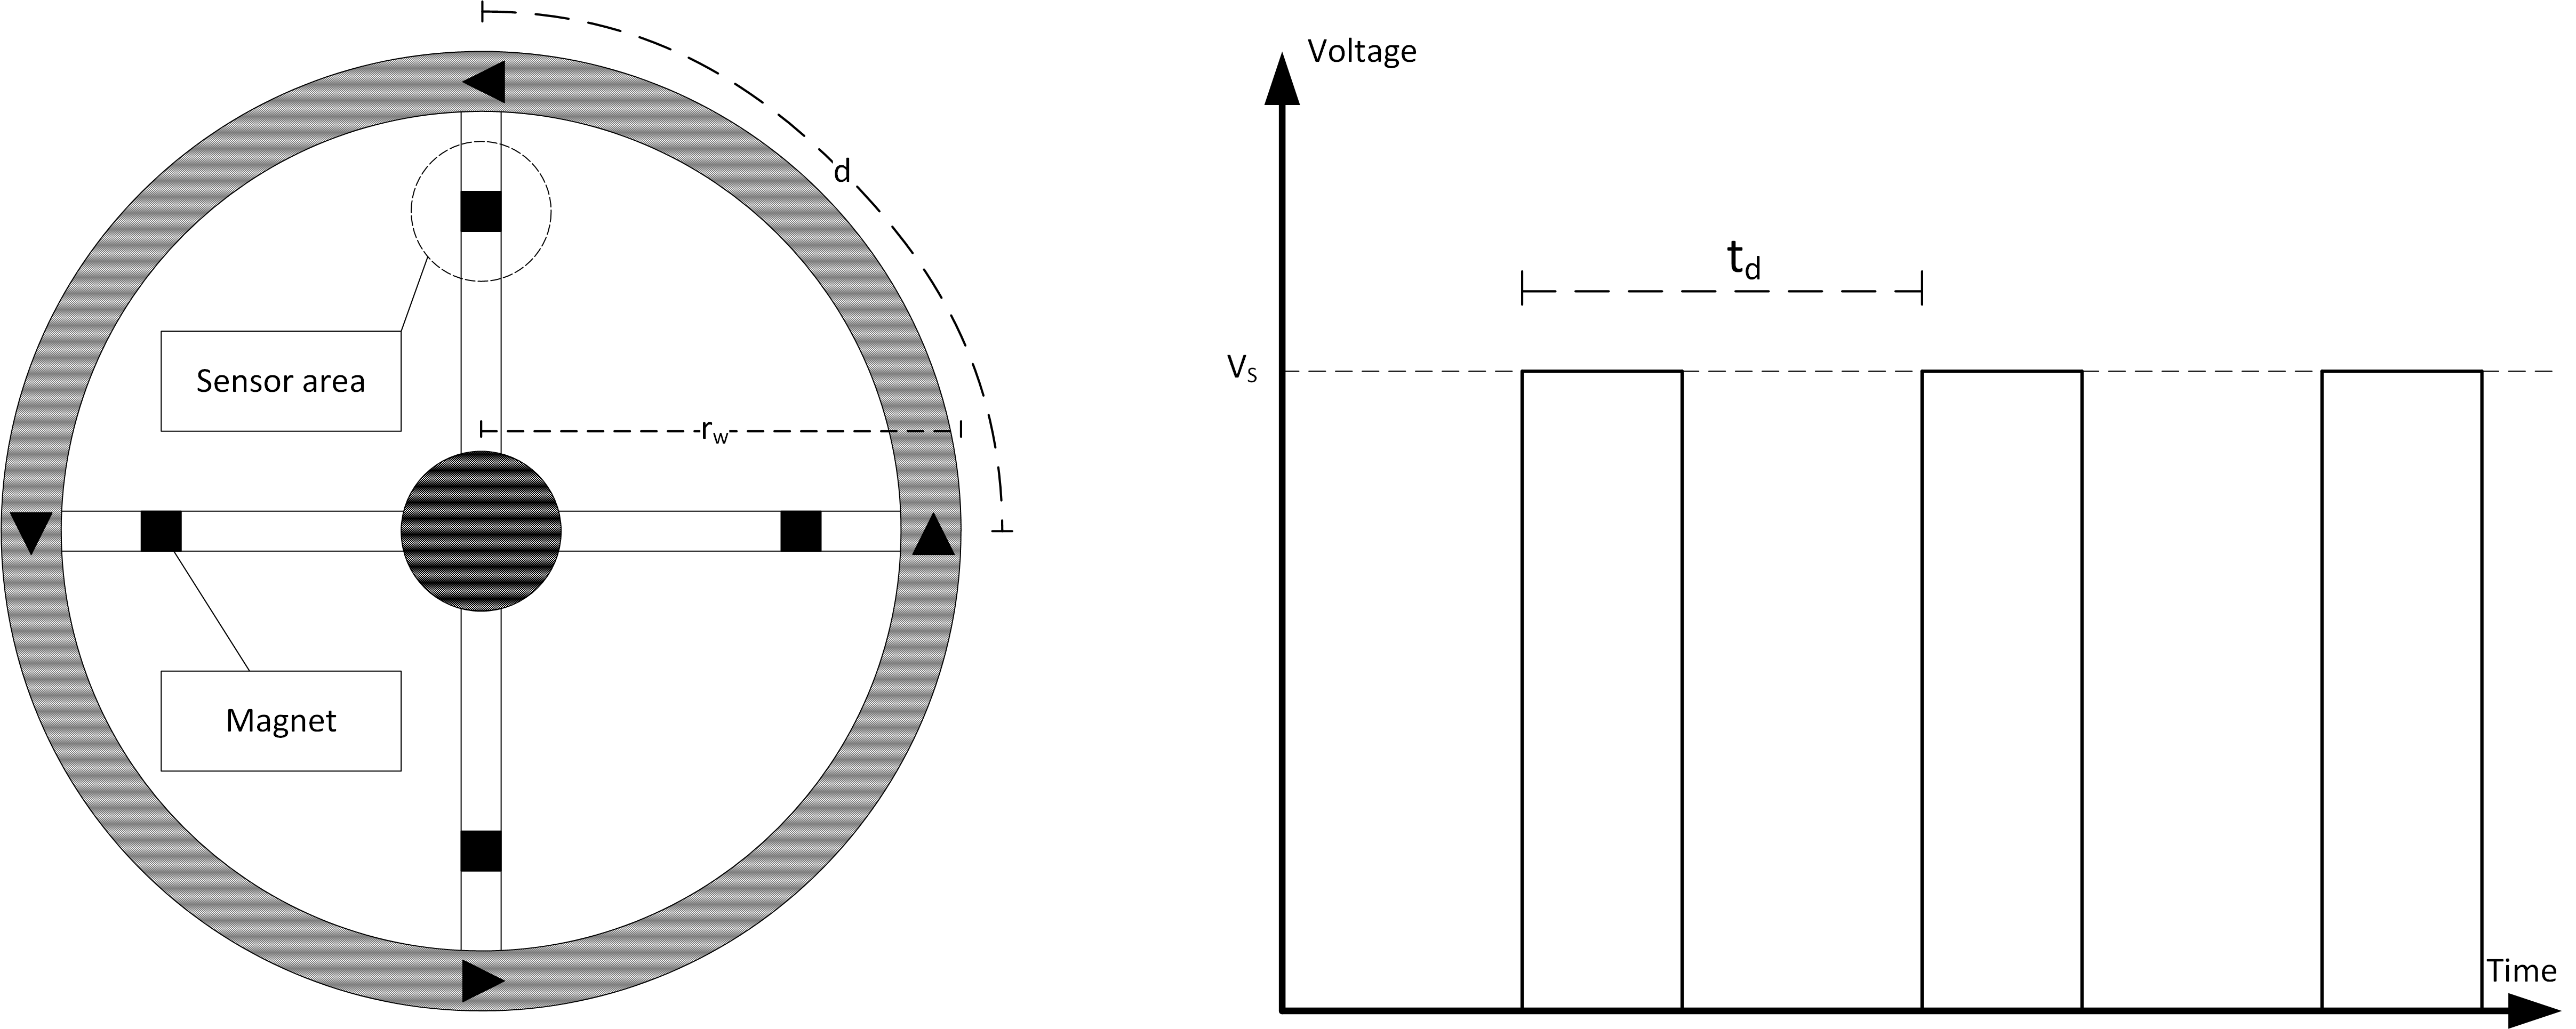
\includegraphics[width=0.9\linewidth]{Hardware/Pictures/Speedometer_Sketch}
	\caption{Speedometer sketch \& sensor output}
	\label{fig:Speed_sketch}
\end{figure}

\newpage
The distance between the rising-edges on the signal is inverse proportional with the car's speed. The distance between each spoke d can be calculated using the wheel's radius r and the number of spokes k on the wheel:
\begin{align}
		d = \frac{2 \cdot r_w \cdot \pi}{k}
\end{align}
This means that during the time between the rising-edges t\textsubscript{d}, the car must have travelled the distance d - if it is assumed that there is no slip between the wheel and the road.\\
The car's velocity v can therefore be calculated as:
\begin{align}
		v &= \frac{d}{t_d}
\end{align}

Neither of the calculations above are completed as the mechanical parts of AU2 wasn't complete during the writing of this documentation. This also results in the fact that the Speedometer hasn't been implemented nor tested. It is, however, the hope that the system can quickly be implemented when the mechanical parts are finished - and that the the speed can be calculated by the PSoC on the fly. 